\documentclass[12pt]{article}

\usepackage[spanish]{babel}
\usepackage[none]{hyphenat}
\usepackage[left=1.5cm, right=1.5cm, top = 2cm, bottom=2.5cm]{geometry}
\usepackage{parskip}
\usepackage[export]{adjustbox}
\usepackage{enumitem}[shortlabels]
\usepackage{listings} 
\usepackage{color}
\usepackage{fancyhdr}
\usepackage{graphicx}
\usepackage{caption} 
% \usepackage{subcaption}
\usepackage{wrapfig}
% \usepackage{longtable}
% \usepackage{multirow, makecell}
% \usepackage{amsmath} 
\usepackage[hidelinks]{hyperref}
\usepackage{csquotes}
\usepackage{tocloft}

\newcommand{\linejump}{\hfill \break}
\renewcommand{\thefootnote}{\fnsymbol{footnote}}
% \newcommand{\unit}[1]{\ensuremath{\, \mathrm{#1}}}

\definecolor{dkgreen}{rgb}{0,0.6,0}
\definecolor{gray}{rgb}{0.5,0.5,0.5}
\definecolor{mauve}{rgb}{0.58,0,0.82}
\lstset{
  language=Java,
  aboveskip=3mm,
  belowskip=3mm,
  showstringspaces=false,
  columns=flexible,
  basicstyle={\scriptsize\ttfamily},
  numbers=none,
  numberstyle=\tiny\color{gray},
  keywordstyle=\color{blue},
  commentstyle=\color{dkgreen},
  stringstyle=\color{mauve},
  breaklines=true,
  breakatwhitespace=true,
  tabsize=2
}

\sloppy
\setlength{\parindent}{0cm}
\setlength{\columnsep}{0.5cm}
\setlength{\cftbeforesecskip}{0.3cm}
\setlength{\cftbeforesubsecskip}{0.2cm}
\setlength{\cftbeforesubsubsecskip}{0.18cm}
\setlength{\cftbeforefigskip}{0.2cm}
\decimalpoint
\graphicspath{{img/}}

\hypersetup{colorlinks=true, urlcolor=blue, citecolor=blue, linkcolor=black}
\urlstyle{same}

\pagestyle{fancyplain}
\fancyhf{}
\fancyhead[L]{\scriptsize 
  Universidad Nacional Autónoma de México \\
  Programación Orientada a Objetos \\
  M.C. Leonardo Ledesma Dominguez
}
\fancyhead[R]{\thepage}

\begin{document}
  \begin{center}
    \linejump
    \LARGE \textbf{Proyecto Final. Primera entrega. Dominó}
  \end{center}

  \begin{flushright}
    \textbf{Integrantes} \\
    Acosta Porcayo Alan Omar 320206102 \\
    Gutiérrez Grimaldo Alejandro 320282098 \\
    Medina Villa Samuel 320249538 
  \end{flushright}

  \tableofcontents
  \listoffigures
  \newpage

  \section{Antecedentes históricos}
  El origen de este juego no es tan claro, ya que algunos historiadores y antropólogos fueron los griegos, también otros afirman que fueron los hebreos. Sin embargo, el juego actual del dominó parece que se inició en China, donde se jugaba hace 1.500 años de manera semejante a como se hace hoy. Se podría considerar como el primer dominó de la historia.
  
  La forma actual conocida en Europa y el mundo no aparece hasta el siglo XVIII, cuando lo introdujeron los italianos en este continente. Gracias a la enorme expansión de la cultura europea a través del mundo, llegó a diversos países y culturas.

  Inicialmente, las fichas se fabricaban mediante la unión de dos láminas de ébano en ambos lados de la ficha de hueso. Este método tenía la ventaja de prevenir posibles trampas al ocultar los puntos en la parte posterior de la ficha bajo ciertas condiciones de iluminación, además de crear un atractivo contraste entre los puntos blancos y el fondo negro, lo que permitía que el hueso fuera visible a través de los agujeros en el ébano.

  \section{Descripción}
  El objetivo principal del juego de dominó es ser el primer jugador en quedarse sin fichas en su mano. Para lograrlo, los jugadores deben emparejar las fichas que poseen con las que ya están en la mesa, asegurándose de que los números de los puntos coincidan. Esto implica tomar decisiones estratégicas sobre cuándo y cómo jugar sus fichas para maximizar sus posibilidades de quedarse sin fichas antes que sus oponentes. 

  \section{Definición de clases}
  \subsection{Clase \textit{Ficha}}
  Esta clase representa una ficha de dominó simple. 

  \subsubsection{Atributos}
  \begin{enumerate}
    \item \textit{caraIzq.} Variable privada de tipo \textit{int} con el valor de la parte izquierda de la ficha.
    \item \textit{caraDer.} Variable privada de tipo \textit{int} con el valor de la parte derecha de la ficha.
    \item \textit{suma.} Variable privada de tipo \textit{int} con la suma de ambas partes de la ficha, se calcula al momento de crear la ficha.
    \item \textit{mula.} Variable privada de tipo \textit{boolean} que indica si la ficha es una mula o no.
  \end{enumerate}

  \subsubsection{Métodos}
  \begin{enumerate}
    \item \textit{Ficha(int caraIzq, int caraDer).} Método constructor que recibe dos enteros que representan los valores de las caras de la ficha. Calcula la suma y determina si la ficha es una mula.
    \item \textit{getCaraIzq().} Método público que retorna el valor de la cara izquierda de la ficha.
    \item \textit{getCaraDer().} Método público que retorna el valor de la cara derecha de la ficha.
    \item \textit{getSuma().} Método público que retorna el valor de la suma de la ficha.
    \item \textit{esMula().} Método público que retorna un booleano que indica si la ficha es una mula o no. 
    \item \textit{girar().} Método público que intercambia los valores de las caras de la ficha.
    \item \textit{toString().} Método público (sobreescritura) que retorna una cadena con formato del valor de las caras de la ficha.
  \end{enumerate}

  \subsection{Clase Abstracta \textit{Jugador}}
  Esta clase representa a un jugador de dominó, ya sea humano o bot.

  \subsubsection{Atributos}
  \begin{enumerate}
    \item \textit{nombre.} Variable protegida de tipo \textit{String} con el nombre del jugador.
    \item \textit{fichas.} Variable protegida de tipo \textit{ArrayList$<$Ficha$>$} con las fichas del jugador.
    \item \textit{puedeJugar.} Variable protegida de tipo \textit{boolean} que indica si el jugador tiene una ficha que pueda jugar.
  \end{enumerate}

  \subsubsection{Métodos}
  \begin{enumerate}
    \item \textit{getNombre().} Método público que retorna el nombre del jugador.
    \item \textit{getFichas().} Método público que retorna las fichas del jugador.
    \item \textit{getFicha(int i).} Método público que retorna la ficha en la posición \textit{i} del jugador.
    \item \textit{getCantidadFichas().} Método público que retorna la cantidad de fichas del jugador.
    \item \textit{agregarFicha(Ficha ficha).} Método público que agrega una ficha a las fichas del jugador.
    \item \textit{puedeJugar().} Método público que retorna un booleano que indica si el jugador puede jugar.
    \item \textit{puedeJugar(ArrayList$<$Ficha$>$ mesaActual).} Método público (sobrecarga) que comprueba si dentro de las fichas del jugador hay alguna que pueda jugarse en la mesa actual y actualiza el valor de \textit{puedeJugar}.
    \item \textit{robar(ArrayList$<$Ficha$>$ pozo).} Método público que sustrae una ficha del pozo y la agrega a las fichas del jugador.
    \item \textit{primerTurno(ArrayList$<$Ficha$>$ mesaActual).} Método público abstracto que realiza el primer turno del jugador.
    \item \textit{turno(ArrayList$<$Ficha$>$ mesaActual).} Método público abstracto que realiza los siguientes turnos del jugador. 
  \end{enumerate}

  \subsection{Clase \textit{Humano}}
  Esta clase representa a un jugador controlado por el usuario.

  \subsubsection{Métodos}
  \begin{enumerate}
    \item \textit{Humano(String nombre).} Método constructor que recibe el nombre del jugador.
    \item \textit{primerTurno(ArrayList$<$Ficha$>$ mesaActual).} Método público (sobreescritura) que realiza el primer turno de manera automática jugando la mula mas alta o si no tiene mula, la ficha con la suma mas alta.
    \item \textit{turno(ArrayList$<$Ficha$>$ mesaActual).} Método público (sobreescritura) que realiza los siguientes turnos por medio de la entrada del usuario. Primero le pide al usuario que elija una ficha dentro del rango de sus fichas, luego le pide que elija un lado de la mesa en el que la quiere colocar y si se introdujeron valores correctos realiza el movimiento, si no, vuelve a pedir los valores.
  \end{enumerate}

  \subsection{Clase \textit{Bot}}
  Esta clase representa a un jugador controlado por la computadora.

  \subsubsection{Métodos}
  \begin{enumerate}
    \item \textit{Bot(String nombre).} Método constructor que recibe el nombre del jugador.
    \item \textit{primerTurno(ArrayList$<$Ficha$>$ mesaActual).} Método público (sobreescritura) que realiza el primer turno de manera automática jugando la mula mas alta o si no tiene mula, la ficha con la suma mas alta.
    \item \textit{turno(ArrayList$<$Ficha$>$ mesaActual).} Método público (sobreescritura) que realiza los siguientes turnos de manera automática buscando una ficha que pueda ser colocada empezando en la parte izquierda de la mesa y si no encuentra, busca en la parte derecha. 
  \end{enumerate}

  \subsection{Clase \textit{Mesa}} 
  Esta clase representa la mesa de juego. 

  \subsubsection{Atributos}
  \begin{enumerate}
    \item \textit{mesa.} Variable privada y estática de tipo \textit{ArrayList$<$Ficha$>$} con las fichas de la mesa.
    \item \textit{pozo.} Variable privada y estática de tipo \textit{ArrayList$<$Ficha$>$} con las fichas sobrantes del juego.
    \item \textit{jugadores.} Variable privada y estática de tipo \textit{List$<$Jugador$>$} con los jugadores del juego. Inicialmente contiene un objeto de tipo \textit{Humano} y dos de tipo \textit{Bot}.
  \end{enumerate}

  \subsubsection{Métodos}
  \begin{enumerate}
    \item \textit{Mesa(int tipoJuego).} Método constructor que crea las fichas de la mesa y las agrega a \textit{mesa}. Determina el tipo de juego entre jugador vs bot o bot vs bot. Mezcla las fichas de la mesa, las reparte entre los jugadores y decide quien empieza.
    \item \textit{getMesa().} Método público que retorna las fichas de la mesa.
    \item \textit{getPozo().} Método público que retorna las fichas del pozo.
    \item \textit{getJugadores().} Método público que retorna los jugadores del juego.
    \item \textit{mezclar().} Método privado que por medio de un número aleatorio intercambia las fichas de la mesa un total de 28 veces. 
    \item \textit{repartir().} Método privado que reparte 7 fichas de la mesa a cada uno de los dos jugadores y las restantes las agrega al pozo.
    \item \textit{decidirPrimerTurno().} Método privado que determina quien empieza el juego buscando quien tiene la mula mas alta y si no hay mula, quien tiene la ficha con la suma mas alta. En caso de que el primer turno sea del jugador en la posición 1 de la lista de jugadores se cambia el orden de los jugadores.
    \item \textit{cambioDeTurno().} Método público que cambia el orden de los jugadores en la lista.
    \item \textit{imprimir().} Método público que imprime el estado actual de la mesa.
    \item \textit{imprimir(ArrayList$<$Ficha$>$ fichas).} Método público (sobrecarga) que imprime las fichas que recibe como parámetro con el número de ficha arriba de cada una.
  \end{enumerate}

  \subsection{Clase \textit{Domino}}
  Esta clase contiene el método \textit{main} y es la encargada de ejecutar la lógica principal del juego, la cual será explicada en la sección de algoritmo.
  
  \section{Definición de objetos}
  \begin{itemize}
    \item \textit{ArrayList$<$Ficha$>$.} Colección de objetos de tipo \textit{Ficha}. Se crea en las clases \textit{Mesa}, \textit{Humano} y \textit{Bot} para almacenar las fichas de la mesa, las fichas del jugador y las fichas que puede jugar el bot respectivamente.
    \item \textit{List$<$Jugador$>$.} Colección de objetos de tipo \textit{Jugador}. En ella se almacenan objetos de tipo \textit{Humano} y \textit{Bot} que representan a los jugadores del juego. Se crea en la clase \textit{Mesa}.
    \item \textit{Mesa.} Objeto de tipo \textit{Mesa} que contiene la configuración inicial del juego. Se crea en la clase \textit{Domino}.
    \item \textit{Scanner.} Objeto de tipo \textit{Scanner} que permite la entrada de datos por parte del usuario. Se crea en la clase \textit{Humano} y \textit{Domino}.
    \item \textit{Clip.} Objeto de tipo \textit{Clip} que la utilización de clips de audio. Se crea en la clase \textit{Domino}.
    \item \textit{ProcessBuilder.} Objeto de tipo \textit{ProcessBuilder} que permite la ejecución de comandos en la terminal. Se crea en la clase \textit{Domino}.
  \end{itemize}

  \section{Algoritmo}
  Se comienza creando un objeto \textit{Scanner} llamado \textit{sc} para leer las entradas del usuario y un objeto \textit{Clip} llamado \textit{musica} para reproducir los clips de audio. Para reproducir un clip se hace dentro de un bloque \textit{try-catch} para evitar que el programa se detenga en caso de que no se encuentre el archivo de audio.

  \begin{lstlisting}
Scanner sc = new Scanner(System.in);
Clip musica = null;

try {
  musica = AudioSystem.getClip();
  musica.open(AudioSystem.getAudioInputStream(Domino.class.getResource("/recursos/MoonlightSonata.wav")));
  musica.loop(Clip.LOOP_CONTINUOUSLY); 
} catch (Exception e) {
  e.printStackTrace();
}
  \end{lstlisting}

  Luego, se imprime el menú con las opciones de juego para que el usuario pueda seleccionar jugador vs bot o bot vs bot. Se lee la entrada del usuario y se crea un objeto de tipo \textit{Mesa} llamado \textit{mesa} con el tipo de juego seleccionado por el usuario.

  \begin{lstlisting}
System.out.println("%%%%%%%%%%%%%%% Bienvenido a Domino %%%%%%%%%%%%%%%");
System.out.println("Escoga el modo de juego:");
System.out.println("1. Jugador vs Bot");
System.out.println("2. Bot vs Bot");
System.out.print("$ ");
int tipoJuego = sc.nextInt();
Mesa mesa = new Mesa(tipoJuego);
  \end{lstlisting}

  Dentro de un ciclo \textit{while} con la condición de repetición de que los jugadores tengan fichas y el pozo no este vacío, se limpia la terminal usando una un bloque \textit{try-catch} y un objeto \textit{ProcessBuilder}.

  \begin{lstlisting}
try {
  new ProcessBuilder("cmd", "/c", "cls").inheritIO().start().waitFor();
} catch (Exception e) {
  e.printStackTrace();
}
  \end{lstlisting}

  Posteriormente, se imprime las fichas de la mesa, el número de fichas en el pozo y se anuncia el turno del jugador en la posición 0 de la lista de jugadores e imprime sus fichas. 

  \begin{lstlisting}
System.out.println("\n\nMesa actual:");
mesa.imprimir();
System.out.println("\nNumero de fichas en el Pozo: " + mesa.getPozo().size());

System.out.println("\n%%%%% Turno de " + mesa.getJugadores().get(0).getNombre() + " %%%%%");
mesa.imprimir(mesa.getJugadores().get(0).getFichas());
  \end{lstlisting}
 
  El siguiente bloque de código corresponde al turno de los jugadores. Si la mesa esta vacia quiere decir que es el primer turno, en ese caso se llama al método \textit{primerTurno} y se continua con el flujo del programa. Para los turnos siguientes primero se comprueba si el jugador puede jugar una ficha realiza su turno con el método \textit{turno}. En caso de que no pueda jugar y no haya fichas en el pozo se imprime un mensaje diciendo que el jugador con el turno actual pasa de turno, y si hay fichas en el pozo roba una, se vuelve a imprimir sus fichas y se pasa de turno. 

  \begin{lstlisting}
if (mesa.getMesa().isEmpty())
  mesa.getJugadores().get(0).primerTurno(mesa.getMesa());
else {
  if (mesa.getJugadores().get(0).puedeJugar(mesa.getMesa())) 
    mesa.getJugadores().get(0).turno(mesa.getMesa());
  else { 
    if (mesa.getPozo().isEmpty()) { 
      System.out.println("No puedes jugar y no hay fichas en el pozo, pasas tu turno");

      try {
        Thread.sleep(3000);
      } catch (InterruptedException e) {
        e.printStackTrace();
      }
    } else {
      if (mesa.getJugadores().get(0) instanceof Humano)
        System.out.println("Necesitas robar una ficha");

      try {
        Thread.sleep(3000);
      } catch (InterruptedException e) {
        e.printStackTrace();
      }

      System.out.println(mesa.getJugadores().get(0).getNombre() + " roba 1 ficha y pasa su turno");
      mesa.getJugadores().get(0).robar(mesa.getPozo());
      mesa.imprimir(mesa.getJugadores().get(0).getFichas());

      try {
        Thread.sleep(3000);
      } catch (InterruptedException e) {
        e.printStackTrace();
      }
    }
  }
}
  \end{lstlisting}

  Al salir del ciclo \textit{while}, dentro de un bloque \textit{try-catch} se para la reproducción del clip de audio y se inicia otro clip de audio con la música de victoria. 

  \begin{lstlisting}
try {
  if (musica != null)
    musica.stop();
  
  musica = AudioSystem.getClip();
  musica.open(AudioSystem.getAudioInputStream(Domino.class.getResource("/recursos/Victoria.wav")));
  musica.start();
} catch (Exception e) {
  e.printStackTrace();
}        
  \end{lstlisting}

  Para terminar se decide el ganador. Si un jugador se queda sin fichas se imprime un mensaje diciendo que gano pero si el pozo se vacía se busca quien tiene la suma más alta y se imprime un mensaje diciendo que gano o si hay empate.

  \begin{lstlisting}
if (!mesa.getJugadores().get(0).puedeJugar() && 
      !mesa.getJugadores().get(1).puedeJugar() &&
      mesa.getPozo().isEmpty() ) {
  int suma1 = 0, suma2 = 0;
  System.out.println("Se acabaron las fichas");

  for (int i = 0; i < mesa.getJugadores().get(0).getCantidadFichas(); i++)
    suma1 += mesa.getJugadores().get(0).getFicha(i).getSuma();
  for (int i = 0; i < mesa.getJugadores().get(1).getCantidadFichas(); i++)
    suma2 += mesa.getJugadores().get(1).getFicha(i).getSuma();
  
  if (suma1 < suma2)
    System.out.println("El ganador es " + mesa.getJugadores().get(0).getNombre());
  else if (suma1 > suma2)
    System.out.println("El ganador es " + mesa.getJugadores().get(1).getNombre());
  else
    System.out.println("Empate");
} else 
  System.out.println("\n%%%%%%%%%% El ganador es " + mesa.getJugadores().get(0).getNombre() + " %%%%%%%%%%");
  \end{lstlisting}

  \section{Herencia de clases}
  La única herencia que realiza es de la clase abstracta \textit{Jugador} a las clases \textit{Humano} y \textit{Bot}. La definición de \textit{Jugador} contiene dos métodos abstractos que son \textit{primerTurno} y \textit{turno} que son implementados en las clases \textit{Humano} y \textit{Bot} respectivamente.

  \section{Conclusiones}


  \section{Referencias}
  De Tenis De Huelva, R. C. R. (s. f.). \textit{Dominó} | \url{https://rcrtenishuelva1889.com/page/9/domino#:~:text=El%20domin%C3%B3%20surgi%C3%B3%20hace%20mil,los%20italianos%20por%20todas%20partes} \\

  Familia Vintage. (2018, June 5). \textit{Como Jugar Al Domino, Reglas del Dominó} [Video]. YouTube. \url{https://www.youtube.com/watch?v=-hbARCT1qow} \\

  Historia, C., $\&$ Historia, C. (2023, 22 abril). \textit{La historia del dominó, es una de las más interesantes que existe Read more}. CurioSfera Historia. \url{https://curiosfera-historia.com/historia-del-domino-origen-inventor/} \\

  \textit{Java Platform SE 8}. (2023). Oracle.com. \url{https://docs.oracle.com/javase/8/docs/api/} \\

  JUEGOS CON HISTORIA: \textit{El Dominó} | Lekotek. (s. f.). \url{https://www.lekotek.org.ar/juegos-con-historia-el-domino/} \\

  Solano, J. (2017, 20 enero). \textit{Manual de prácticas de Programación Orientada a Objetos}. Laboratorio de Computación Salas A y B. \url{http://lcp02.fi-b.unam.mx/} 

  \newpage
  \section{Apéndice}
  \subsection{Diagramas UML de clases}
  \begin{figure}[h!]
    \centering
    \begin{minipage}[l]{0.45\textwidth}
      \centering
      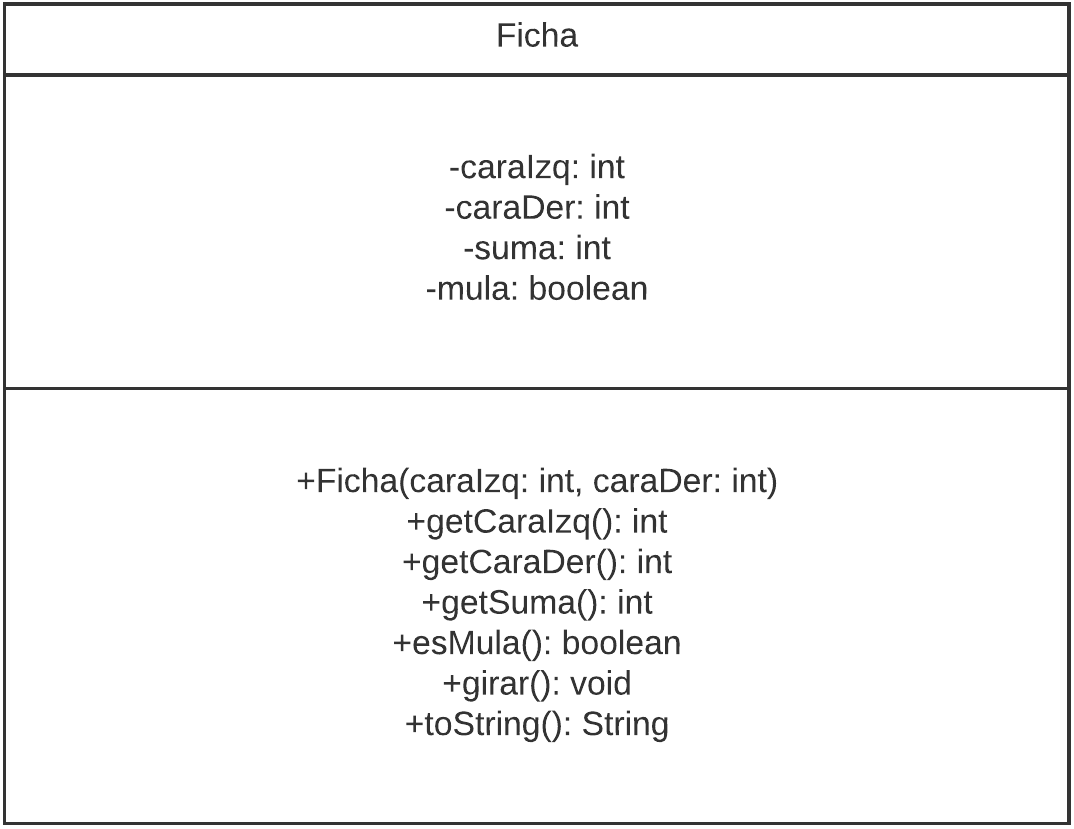
\includegraphics[height=5.5cm]{uml1.png}
      \caption{UML de clase \textit{Ficha}}
    \end{minipage}
    \begin{minipage}[r]{0.45\textwidth}
      \centering
      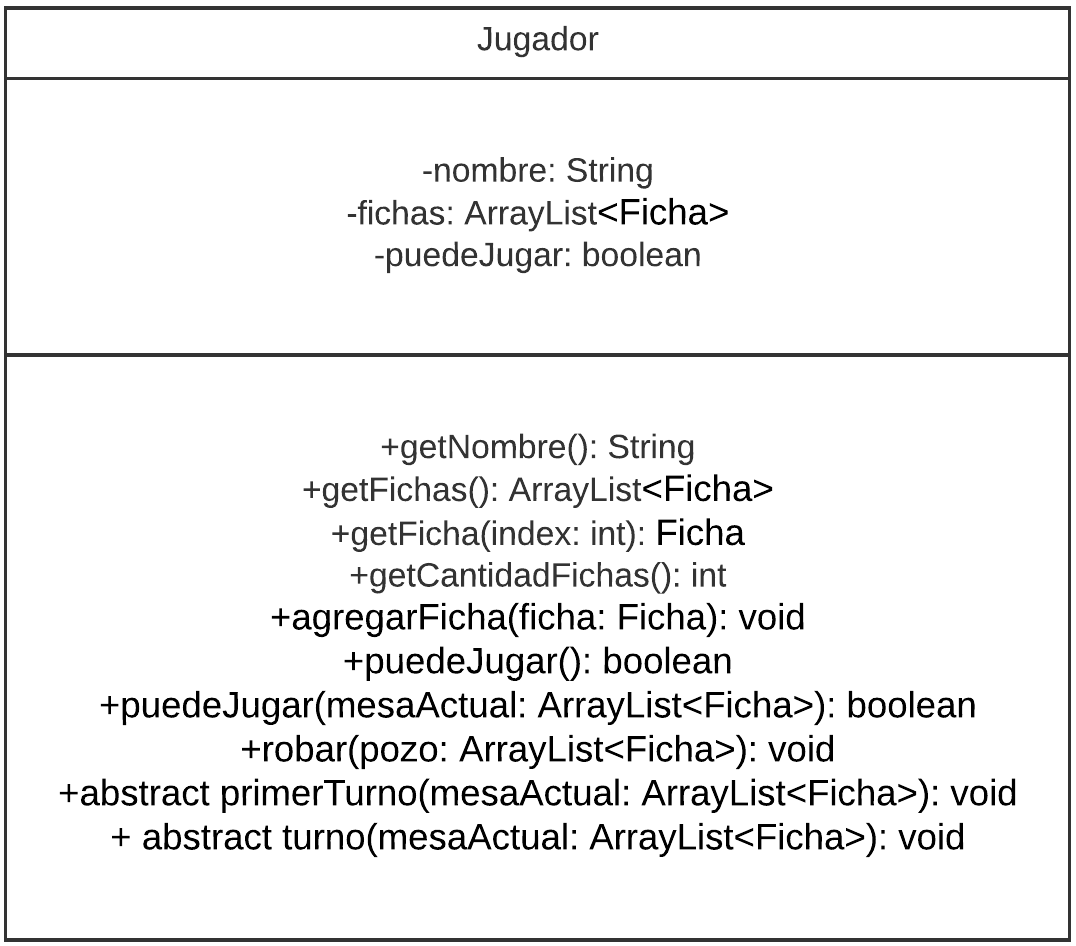
\includegraphics[height=5.5cm]{uml2.png}
      \caption{UML de clase \textit{Jugador}}
    \end{minipage}
  \end{figure}

  \begin{figure}[h!]
    \centering
    \begin{minipage}[l]{0.45\textwidth}
      \centering
      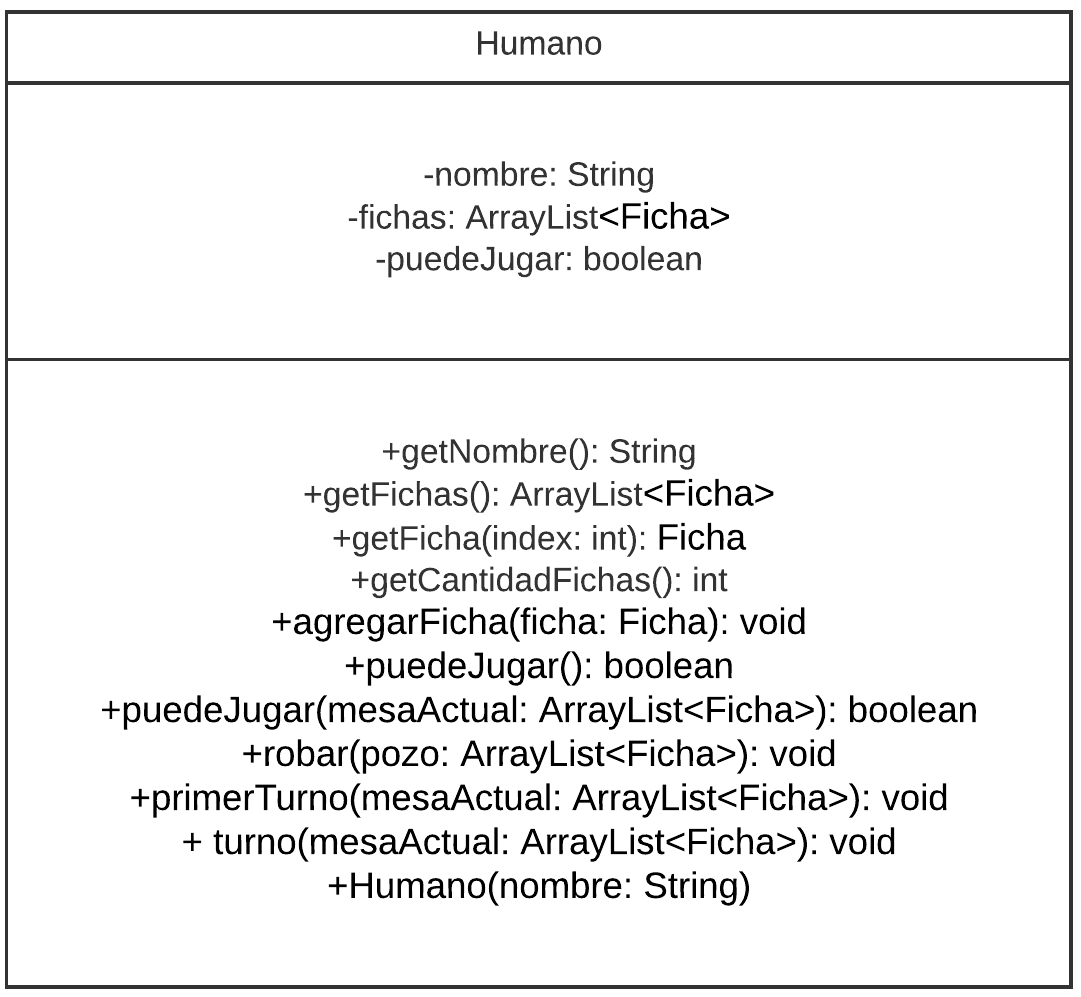
\includegraphics[height=5.5cm]{uml3.png}
      \caption{UML de clase \textit{Humano}}
    \end{minipage}
    \begin{minipage}[r]{0.45\textwidth}
      \centering
      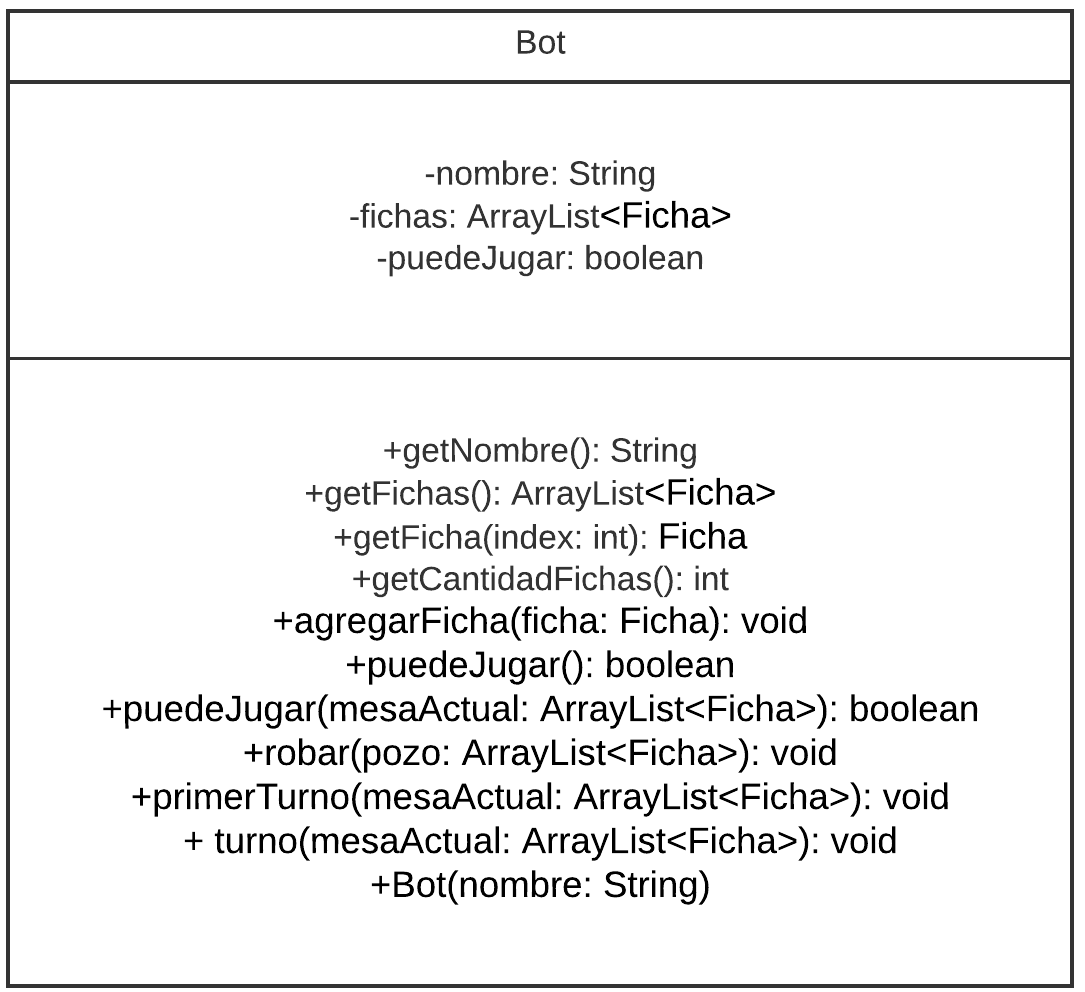
\includegraphics[height=5.5cm]{uml4.png}
      \caption{UML de clase \textit{Bot}}
    \end{minipage}
  \end{figure}

  \begin{figure}[h!]
    \centering
    \begin{minipage}[l]{0.45\textwidth}
      \centering
      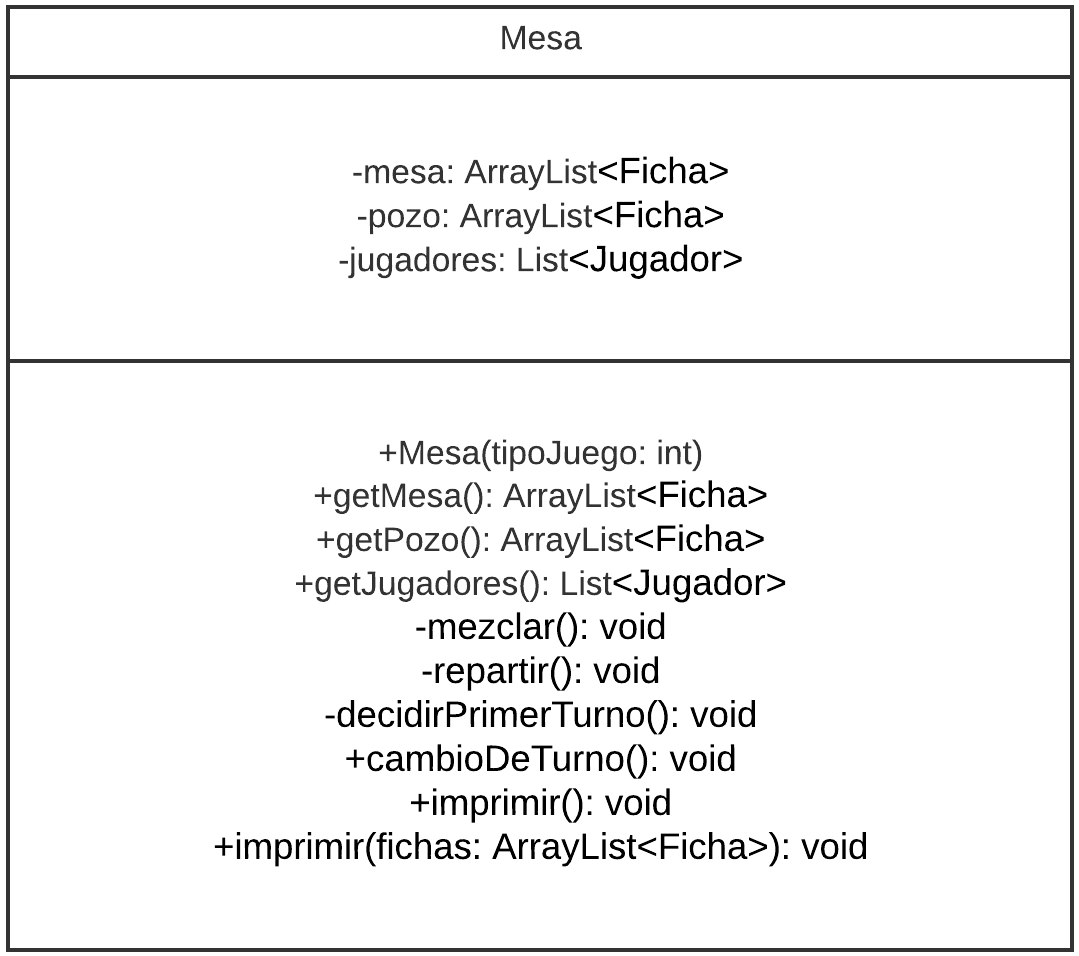
\includegraphics[height=5.5cm]{uml5.png}
      \caption{UML de clase \textit{Mesa}}
    \end{minipage}
    \begin{minipage}[r]{0.45\textwidth}
      \centering
      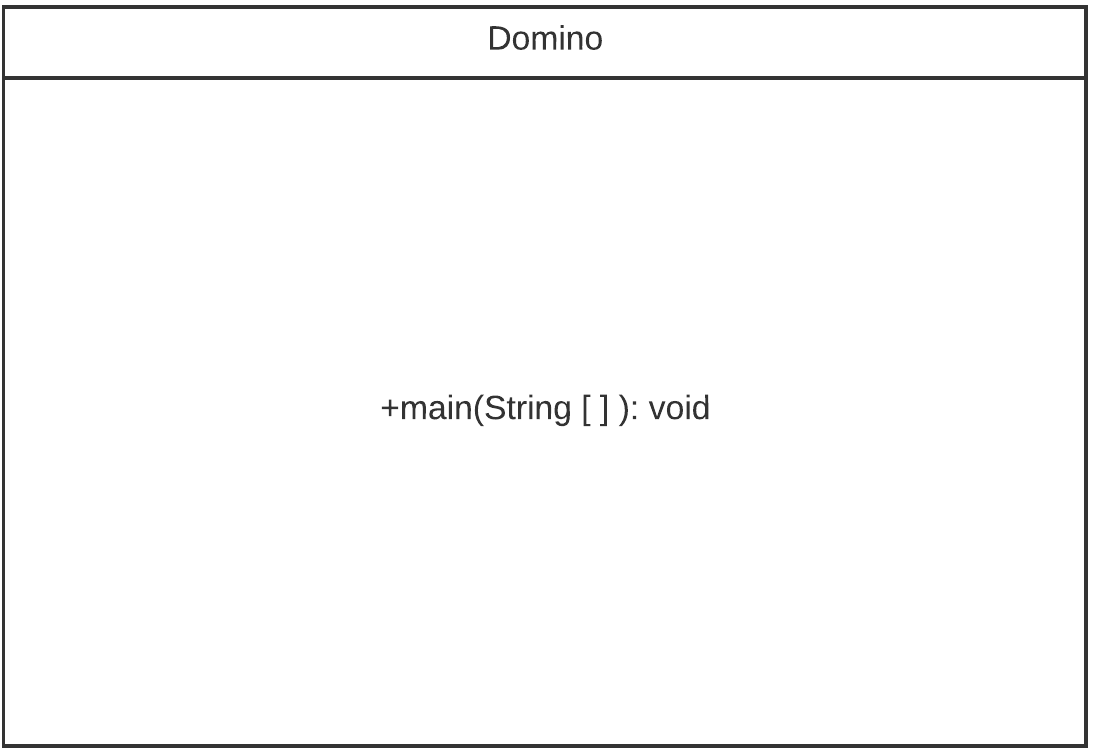
\includegraphics[height=5.5cm]{uml6.png}
      \caption{UML de clase \textit{Domino}} 
    \end{minipage}
  \end{figure}

  \linejump

  \subsection{Diagramas UML de objetos}


  \subsection{Diagrama UML de casos de uso}


  \subsection{Código fuente}
  \subsubsection{Ficha.java}
  \begin{lstlisting}
package domino;

/**
  * Esta clase representa una ficha de domino con dos caras
  */

public class Ficha {
  private int caraIzq;
  private int caraDer;
  private int suma;
  private boolean mula = false;

  /**
    * Metodo constructor que recibe las dos caras de la ficha
    * @param caraIzq El numero de la cara izquierda
    * @param caraDer El numero de la cara derecha
    */
  public Ficha(int caraIzq, int caraDer) {
    this.caraIzq = caraIzq;
    this.caraDer = caraDer;
    this.suma = caraIzq + caraDer;
    if (caraIzq == caraDer)
      mula = true;
  }

  /**
    * Metodo getter para la cara izquierda
    * @return Numero de la cara izquierda
    */
  public int getCaraIzq() {
    return caraIzq;
  }

  /**
    * Metodo getter para la cara derecha
    * @return Numero de la cara derecha
    */
  public int getCaraDer() {
    return caraDer;
  }

  /**
    * Metodo getter para la suma de las caras
    * @return Suma de las caras
    */
  public int getSuma() {
    return suma;
  }

  /**
    * Metodo getter para saber si la ficha es mula
    * @return true si la ficha es mula, false si no
    */
  public boolean esMula() {
    return mula;
  }

  /**
    * Cambia la cara izquierda por la derecha y viceversa
    */
  public void girar() {
    int aux = caraIzq;
    caraIzq = caraDer;
    caraDer = aux;
  }

  /**
    * Imprime la ficha con el formato [caraIzq|caraDer]
    */
  public String toString() {
    return "[" + caraIzq + "|" + caraDer + "]";
  }
}
  \end{lstlisting}

  \subsubsection{Jugador.java}
  \begin{lstlisting}
package domino;

import java.util.ArrayList;

/**
  * Esta clase abstracta representa un jugador de domino
  */

public abstract class Jugador {
  protected String nombre;
  protected ArrayList<Ficha> fichas = new ArrayList<Ficha>();
  protected boolean puedeJugar = true;

  /**
    * Metodo getter para el nombre del jugador
    * @return Nombre del jugador
    */
  public String getNombre() {
    return nombre;
  }

  /**
    * Metodo getter para las fichas del jugador
    * @return Fichas del jugador
    */
  public ArrayList<Ficha> getFichas() {
    return fichas;
  }

  /**
    * Metodo getter para una ficha especifica del jugador
    * @param i Indice de la ficha
    * @return Ficha del jugador
    */
  public Ficha getFicha(int i) {
    return fichas.get(i);
  }
  
  /**
    * Metodo getter para la cantidad de fichas del jugador
    * @return Cantidad de fichas del jugador
    */
  public int getCantidadFichas() {
    return fichas.size();
  }
  
  /**
    * Agrega una ficha a las fichas del jugador
    * @param ficha Ficha a agregar
    */
  public void agregarFicha(Ficha ficha) {
    fichas.add(ficha);
  }

  /**
    * Metodo getter para saber si el jugador puede jugar
    * @return true si el jugador puede jugar, false si no
    */
  public boolean puedeJugar() {
    return puedeJugar;
  }

  /**
    * Metodo setter para saber si el jugador puede jugar
    * @param mesaActual La fichas de la mesa actual
    * @return puedeJugar true si el jugador puede jugar, false si no
    */
  public boolean puedeJugar(ArrayList<Ficha> mesaActual) {
    for (Ficha ficha : fichas) {
      if (ficha.getCaraIzq() == mesaActual.get(0).getCaraIzq() || 
              ficha.getCaraDer() == mesaActual.get(0).getCaraIzq() || 
              ficha.getCaraIzq() == mesaActual.get(mesaActual.size() - 1).getCaraDer() || 
              ficha.getCaraDer() == mesaActual.get(mesaActual.size() - 1).getCaraDer()) {
        puedeJugar = true;    
        return puedeJugar;
      }
    }
    puedeJugar = false;
    return puedeJugar;
  }

  /**
    * Metodo para robar una ficha del pozo
    * @param pozo El pozo de fichas
    */
  public void robar(ArrayList<Ficha> pozo) {
    fichas.add(pozo.get(0));
    pozo.remove(0);
  }

  /**
    * Metodo abstracto para el primer turno del jugador
    * @param mesaActual La fichas de la mesa actual
    */
  public abstract void primerTurno(ArrayList<Ficha> mesaActual);

  /**
    * Metodo abstracto para el turno del jugador
    * @param mesaActual La fichas de la mesa actual
    */
  public abstract void turno(ArrayList<Ficha> mesaActual);
}
  \end{lstlisting}

  \subsubsection{Humano.java}
  \begin{lstlisting}
package domino;

import java.util.ArrayList;
import java.util.Scanner;

/**
 * Esta clase representa un jugador humano de domino
 */

public class Humano extends Jugador {
  /**
    * Metodo constructor
    * @param nombre Nombre del jugador
    */
  public Humano(String nombre) {
    this.nombre = nombre;
  }

  /**
    * Metodo para el primer turno del jugador
    * @param mesaActual Mesa actual del juego
    */
  @Override
  public void primerTurno(ArrayList<Ficha> mesaActual) {
    Scanner sc = new Scanner(System.in);
    int ficha = -1;
    int max = -1;

    for (Ficha f : fichas) {
      if (f.esMula() && f.getSuma() > max) {
        max = f.getSuma();
        ficha = fichas.indexOf(f);
      }
    }

    if (ficha != -1) 
      System.out.println(nombre + " juegas la mula mas alta: " + fichas.get(ficha));
    else {  
      for (int i = 0; i < fichas.size(); i++) {
        if (fichas.get(i).getSuma() > max) {
          max = fichas.get(i).getSuma();
          ficha = i;
        }
      }
      System.out.println(nombre + " juegas la ficha mas alta: " + fichas.get(ficha));
    }

    mesaActual.add(fichas.get(ficha));
    fichas.remove(ficha);
    
    try {
      Thread.sleep(3000);
    } catch (InterruptedException e) {
      e.printStackTrace();
    }
  }

  /**
    * Metodo para el turno del jugador
    * @param mesaActual Mesa actual del juego
    */
  @Override
  public void turno(ArrayList<Ficha> mesaActual) {
    Scanner sc = new Scanner(System.in);
    int ficha = 0;
    char lado = ' ';
      
    do {
      do {
        System.out.println("Que ficha quieres jugar? (1 - " + fichas.size() + ")");
        ficha = sc.nextInt() - 1;
        if (ficha < 0 || ficha >= fichas.size())
          System.out.println("Ficha invalida");
      } while (ficha < 0 || ficha >= fichas.size());

      System.out.println("Donde la quieres jugar? (izquierda o derecha)");
      lado = sc.next().charAt(0);
      lado = Character.toLowerCase(lado);
      
      if (lado == 'i') {
        if (fichas.get(ficha).getCaraIzq() == mesaActual.get(0).getCaraIzq()) {
          fichas.get(ficha).girar();
          mesaActual.add(0, fichas.get(ficha));
          fichas.remove(ficha); 
          return;
        } else if (fichas.get(ficha).getCaraDer() == mesaActual.get(0).getCaraIzq()) {
          mesaActual.add(0, fichas.get(ficha));
          fichas.remove(ficha);
          return;
        }
      } else if (lado == 'd') {
        if (fichas.get(ficha).getCaraIzq() == mesaActual.get(mesaActual.size() - 1).getCaraDer()) {
          mesaActual.add(fichas.get(ficha));
          fichas.remove(ficha);
          return;
        } else if (fichas.get(ficha).getCaraDer() == mesaActual.get(mesaActual.size() - 1).getCaraDer()) {
          fichas.get(ficha).girar();
          mesaActual.add(fichas.get(ficha));
          fichas.remove(ficha);
          return;
        }
      }

      System.out.println("No puedes jugar esa ficha. Intenta de nuevo.");
    } while (true);
  }
}
  \end{lstlisting}

  \subsubsection{Bot.java}
  \begin{lstlisting}
package domino;

import java.util.ArrayList;

/**
 * Esta clase representa un jugador bot de domino
 */

public class Bot extends Jugador {
  /**
    * Metodo constructor
    * @param nombre Nombre del bot
    */
  public Bot(String nombre) {
    this.nombre = nombre;
  }

  /**
    * Metodo para el primer turno del bot
    * @param mesaActual Mesa actual del juego
    */
  @Override
  public void primerTurno(ArrayList<Ficha> mesaActual) {
    int ficha = -1;
    int max = -1;

    for (Ficha f : fichas) {
      if (f.esMula() && f.getSuma() > max) {
        max = f.getSuma();
        ficha = fichas.indexOf(f);
      }
    }

    if (ficha != -1) 
      System.out.println(nombre + " juega la mula mas alta: " + fichas.get(ficha));
    else { 
      for (int i = 0; i < fichas.size(); i++) {
        if (fichas.get(i).getSuma() > max) {
          max = fichas.get(i).getSuma();
          ficha = i;
        }
      }
      System.out.println(nombre + " juega la ficha mas alta: " + fichas.get(ficha));
    }

    mesaActual.add(fichas.get(ficha));
    fichas.remove(ficha);
    
    try {
      Thread.sleep(3000);
    } catch (InterruptedException e) {
      e.printStackTrace();
    }
  }

  /**
    * Metodo para el turno del bot
    * @param mesaActual Mesa actual del juego
    */
  @Override
  public void turno(ArrayList<Ficha> mesaActual) {
    try {
      Thread.sleep(3000);
    } catch (InterruptedException e) {
      e.printStackTrace();
    }    

    for (int i = 0; i < fichas.size(); i++) {
      if (fichas.get(i).getCaraIzq() == mesaActual.get(0).getCaraIzq()) {
        fichas.get(i).girar();
        mesaActual.add(0, fichas.get(i));
        System.out.println(nombre + " juega " + fichas.get(i) + " a la izquierda");
        fichas.remove(i); 
        break;
      } else if (fichas.get(i).getCaraDer() == mesaActual.get(0).getCaraIzq()) {
        mesaActual.add(0, fichas.get(i));
        System.out.println(nombre + " juega " + fichas.get(i) + " a la izquierda");
        fichas.remove(i);
        break;
      } else if (fichas.get(i).getCaraIzq() == mesaActual.get(mesaActual.size() - 1).getCaraDer()) {
        mesaActual.add(fichas.get(i));
        System.out.println(nombre + " juega " + fichas.get(i) + " a la derecha");
        fichas.remove(i);
        break;
      } else if (fichas.get(i).getCaraDer() == mesaActual.get(mesaActual.size() - 1).getCaraDer()) {
        fichas.get(i).girar();
        mesaActual.add(fichas.get(i));
        System.out.println(nombre + " juega " + fichas.get(i) + " a la derecha");
        fichas.remove(i);
        break;
      }
    }

    try {
      Thread.sleep(3000);
    } catch (InterruptedException e) {
      e.printStackTrace();
    }   
  }
}
  \end{lstlisting}

  \subsubsection{Mesa.java}
  \begin{lstlisting}
package domino;

import java.util.ArrayList;
import java.util.List;
import java.util.Random;

/**
 * Esta clase representa la mesa de juego
 */

public class Mesa {
  private static ArrayList<Ficha> mesa = new ArrayList<Ficha>();
  private static ArrayList<Ficha> pozo = new ArrayList<Ficha>();
  private static List<Jugador> jugadores = new ArrayList<Jugador>() {{
    add(new Humano("Jugador 1"));
    add(new Bot("Bot 1"));
    add(new Bot("Bot 2"));
  }};
  
  /**
    * Metodo constructor
    * @param tipoJuego Tipo de juego (1: Jugador vs Bot, 2: Bot vs Bot)
    */
  public Mesa(int tipoJuego) {
    for (int i = 0; i <= 6; i++) 
      for (int j = i; j <= 6; j++) 
        mesa.add(new Ficha(i, j));
    this.mezclar();

    if (tipoJuego == 1)  
      jugadores.remove(2);
    else if (tipoJuego == 2)
      jugadores.remove(0);

    this.repartir(); 
    this.decidirPrimerTurno();
    mesa.clear(); 
  }

  /**
    * Metodo getter para las fichas de la mesa
    * @return Fichas de la mesa
    */
  public ArrayList<Ficha> getMesa() {
    return mesa;
  }

  /**
    * Metodo getter para las fichas del pozo
    * @return Fichas del pozo
    */
  public ArrayList<Ficha> getPozo() {
    return pozo;
  }

  /**
    * Metodo getter para el ArrayList de jugadores
    * @return Jugadores
    */
  public List<Jugador> getJugadores() {
    return jugadores;
  }

  /**
    * Metodo para mezclar las fichas de la mesa
    */
  private void mezclar() {
    Random random = new Random();
    for (int i = 0; i < mesa.size(); i++) {
      int j = random.nextInt(mesa.size());
      Ficha aux = mesa.get(i);
      mesa.set(i, mesa.get(j));
      mesa.set(j, aux);
    }
  }

  /**
    * Metodo para repartir 7 fichas a cada jugador
    */
  private void repartir() {
    for (int i = 0; i < 7; i++) {
      jugadores.get(0).agregarFicha(mesa.get(i));
      jugadores.get(1).agregarFicha(mesa.get(i + 7));
    }
    for (int i = 14; i < mesa.size(); i++) 
      pozo.add(mesa.get(i));
  }

  /**
    * Metodo para decidir quien empieza el juego
    */
  private void decidirPrimerTurno() {
    int max = -1, mano = -1;

    // Busca la mula con el numero mas alto
    for (int i = 0; i < 7; i ++) { 
      if (jugadores.get(0).getFicha(i).esMula() && jugadores.get(0).getFicha(i).getSuma() > max) {
        max = jugadores.get(0).getFicha(i).getSuma();
        mano = 0;
      }
      if (jugadores.get(1).getFicha(i).esMula() && jugadores.get(1).getFicha(i).getSuma() > max) {
        max = jugadores.get(1).getFicha(i).getSuma();
        mano = 1;
      }
    }

    if (mano != -1) {
      if (mano == 1)
        cambioDeTurno();
      return;
    }
    
    max = -1;
    for (int i = 0; i < 7; i ++) {
      if (jugadores.get(0).getFicha(i).getSuma() > max) {
        max = jugadores.get(0).getFicha(i).getSuma();
        mano = 0;
      }
      if (jugadores.get(1).getFicha(i).getSuma() > max) {
        max = jugadores.get(1).getFicha(i).getSuma();
        mano = 1;
      }
    }

    if (mano == 1)
      cambioDeTurno();
  }

  /**
    * Metodo para cambiar el turno de los jugadores
    */
  public void cambioDeTurno() {
    Jugador aux = jugadores.get(1);
    jugadores.set(1, jugadores.get(0));
    jugadores.set(0, aux);
  }

  /**
    * Metodo para imprimir las fichas de la mesa
    */
  public void imprimir() {
    for (Ficha ficha : mesa)
      System.out.print(ficha + "\t");
    System.out.println();
  }

  /**
    * Metodo para imprimir las fichas de un ArrayList
    * @param fichas ArrayList de fichas
    */
  public void imprimir(ArrayList<Ficha> fichas) {
    for (int i = 1; i <= fichas.size(); i++)
      System.out.print("  " + i + "\t");
    System.out.println();

    for (Ficha ficha : fichas)
      System.out.print(ficha + "\t");
    System.out.println();
  }    
}
  \end{lstlisting}

  \subsubsection{Domino.java}
  \begin{lstlisting}
package domino;

import java.util.Scanner;

import javax.sound.sampled.AudioSystem;
import javax.sound.sampled.Clip;

/**
 * Esta clase representa el juego de domino
 */

public class Domino {
  /**
    * Metodo main.
    * Contiene la logica del juego.
    * @param args Argumentos de la linea de comandos
    */
  public static void main(String[] args) {
    Scanner sc = new Scanner(System.in);
    Clip musica = null;

    try {
      musica = AudioSystem.getClip();
      musica.open(AudioSystem.getAudioInputStream(Domino.class.getResource("/recursos/MoonlightSonata.wav")));
      musica.loop(Clip.LOOP_CONTINUOUSLY); 
    } catch (Exception e) {
      e.printStackTrace();
    }

    System.out.println("%%%%%%%%%%%%%%% Bienvenido a Domino %%%%%%%%%%%%%%%");
    System.out.println("Escoga el modo de juego:");
    System.out.println("1. Jugador vs Bot");
    System.out.println("2. Bot vs Bot");
    System.out.print("$ ");
    int tipoJuego = sc.nextInt();
    Mesa mesa = new Mesa(tipoJuego);

    while ((mesa.getJugadores().get(0).puedeJugar() || 
            mesa.getJugadores().get(1).puedeJugar()) || 
            !mesa.getPozo().isEmpty()) {
      try {
        new ProcessBuilder("cmd", "/c", "cls").inheritIO().start().waitFor();
      } catch (Exception e) {
        e.printStackTrace();
      }

      System.out.println("\n\nMesa actual:");
      mesa.imprimir();
      System.out.println("\nNumero de fichas en el Pozo: " + mesa.getPozo().size());
      
      System.out.println("\n%%%%% Turno de " + mesa.getJugadores().get(0).getNombre() + " %%%%%");
      mesa.imprimir(mesa.getJugadores().get(0).getFichas());

      if (mesa.getMesa().isEmpty())
        mesa.getJugadores().get(0).primerTurno(mesa.getMesa());
      else {
        if (mesa.getJugadores().get(0).puedeJugar(mesa.getMesa())) 
            mesa.getJugadores().get(0).turno(mesa.getMesa());
        else { 
          if (mesa.getPozo().isEmpty()) { 
            System.out.println("No puedes jugar y no hay fichas en el pozo, pasas tu turno");

            try {
              Thread.sleep(3000);
            } catch (InterruptedException e) {
              e.printStackTrace();
            }
          } else {
            if (mesa.getJugadores().get(0) instanceof Humano)
                System.out.println("Necesitas robar una ficha");

            try {
              Thread.sleep(3000);
            } catch (InterruptedException e) {
              e.printStackTrace();
            }

            System.out.println(mesa.getJugadores().get(0).getNombre() + " roba 1 ficha y pasa su turno");
            mesa.getJugadores().get(0).robar(mesa.getPozo());
            mesa.imprimir(mesa.getJugadores().get(0).getFichas());

            try {
              Thread.sleep(3000);
            } catch (InterruptedException e) {
              e.printStackTrace();
            }
          }
        }
      }
      
      if (mesa.getJugadores().get(0).getCantidadFichas() == 0) {
        System.out.println("\n\nMesa final:");
        mesa.imprimir(mesa.getMesa());
        break;
      }

      mesa.cambioDeTurno();
    }
    
    try {
      if (musica != null)
        musica.stop();
      
      musica = AudioSystem.getClip();
      musica.open(AudioSystem.getAudioInputStream(Domino.class.getResource("/recursos/Victoria.wav")));
      musica.start();
    } catch (Exception e) {
      e.printStackTrace();
    }        

    if (!mesa.getJugadores().get(0).puedeJugar() && 
            !mesa.getJugadores().get(1).puedeJugar() &&
            mesa.getPozo().isEmpty() ) {
      int suma1 = 0, suma2 = 0;
      System.out.println("Se acabaron las fichas");

      for (int i = 0; i < mesa.getJugadores().get(0).getCantidadFichas(); i++)
        suma1 += mesa.getJugadores().get(0).getFicha(i).getSuma();
      for (int i = 0; i < mesa.getJugadores().get(1).getCantidadFichas(); i++)
        suma2 += mesa.getJugadores().get(1).getFicha(i).getSuma();
      
      if (suma1 < suma2)
        System.out.println("El ganador es " + mesa.getJugadores().get(0).getNombre());
      else if (suma1 > suma2)
        System.out.println("El ganador es " + mesa.getJugadores().get(1).getNombre());
      else
        System.out.println("Empate");
    } else 
      System.out.println("\n%%%%%%%%%% El ganador es " + mesa.getJugadores().get(0).getNombre() + " %%%%%%%%%%");
    
    try {
      Thread.sleep(5000);
    } catch (InterruptedException e) {
      e.printStackTrace();
    } 

    sc.close();
  }
}
  \end{lstlisting}

  \subsection{Pruebas de funcionamiento}
  Ejecutando el archivo \textit{Domino.jar} con el comando \textit{java -jar Domino.jar} se muestra el menú de opciones de juego. 

  \begin{figure}[h!]
    \centering
    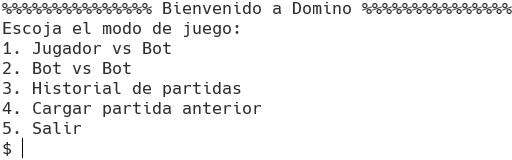
\includegraphics[]{pf1.png}
    \caption{Menú de opciones de juego}
  \end{figure}

  Al seleccionar una opción se limpia la terminal y se inicia el juego tirando la mula más alta o la ficha más alta.

  \begin{figure}[h!]
    \centering
    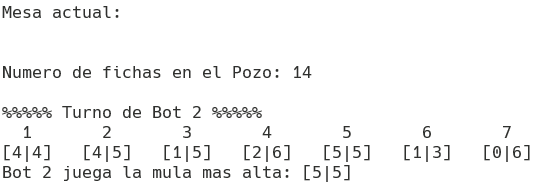
\includegraphics{pf2.png}
    \caption{Inicio del juego}
  \end{figure}
  
  Los siguientes turnos son diferentes dependiendo del tipo de jugador. En caso de que sea un bot se espera 3 segundos antes de que juegue su ficha. En caso de que sea un jugador humano se le pide que seleccione la ficha que quiere jugar y el lado donde la quiere jugar.

  \begin{figure}[h!]
    \centering
    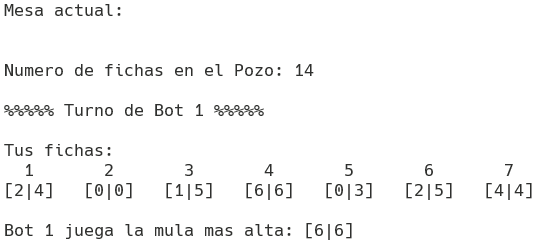
\includegraphics{pf3.png}
    \caption{Turno de jugador Humano}
  \end{figure}

  \begin{figure}[h!]
    \centering
    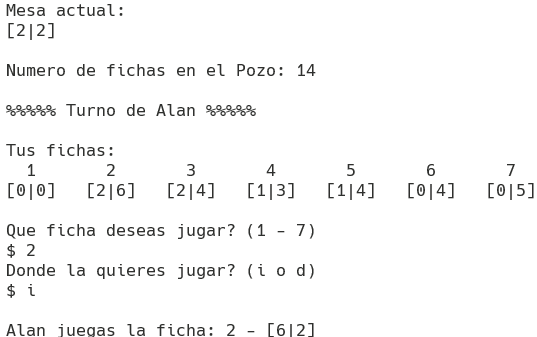
\includegraphics{pf4.png}
    \caption{Turno de jugador Bot}
  \end{figure}

  En caso de que un jugador necesite robar una ficha se muestra un mensaje diciendo y se vuelven a imprimir sus fichas.

  \begin{figure}[h!]
    \centering
    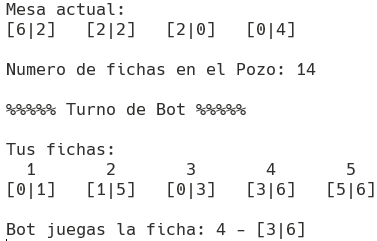
\includegraphics{pf5.png}
    \caption{Mensaje de robar ficha} 
  \end{figure}

  Al ganar el jugador se muestra un mensaje de victoria y se termina el programa.

  \begin{figure}[h!]
    \centering
    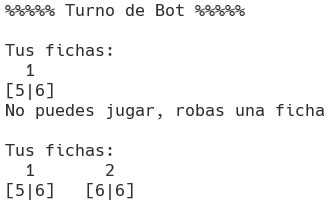
\includegraphics[scale=0.8]{pf6.png}
    \caption{Mensaje de victoria}
  \end{figure}

  \subsection{Documentación de JavaDoc}
  Al ejecutar el comando \textit{javadoc -d documentacion domino/*.java} se genera la documentación de JavaDoc en la carpeta \textit{documentacion}. Algunos ejemplos de la documentación generada se muestran a continuación y lo restante se encuentra en la dirección \url{https://documentacion-domino.netlify.app}.

  \begin{figure}[h!]
    \centering
    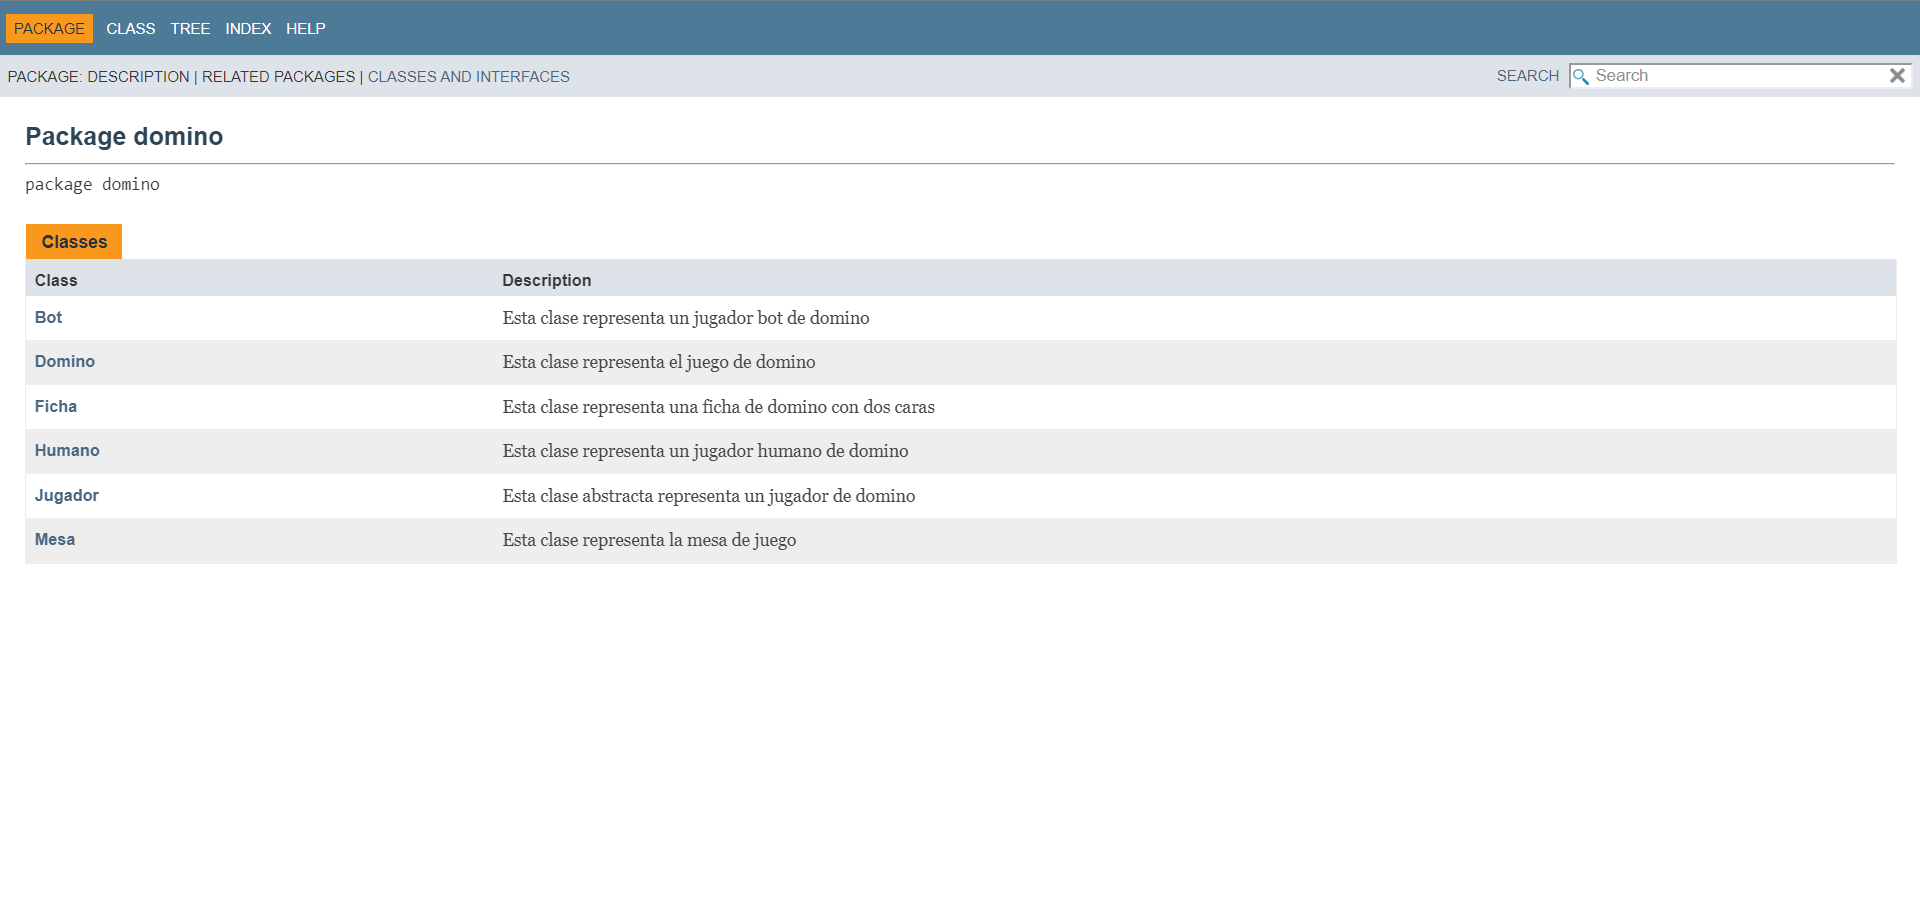
\includegraphics[width=\textwidth]{doc1.png}
    \caption{Página principal}
  \end{figure}

  \begin{figure}[h!]
    \centering
    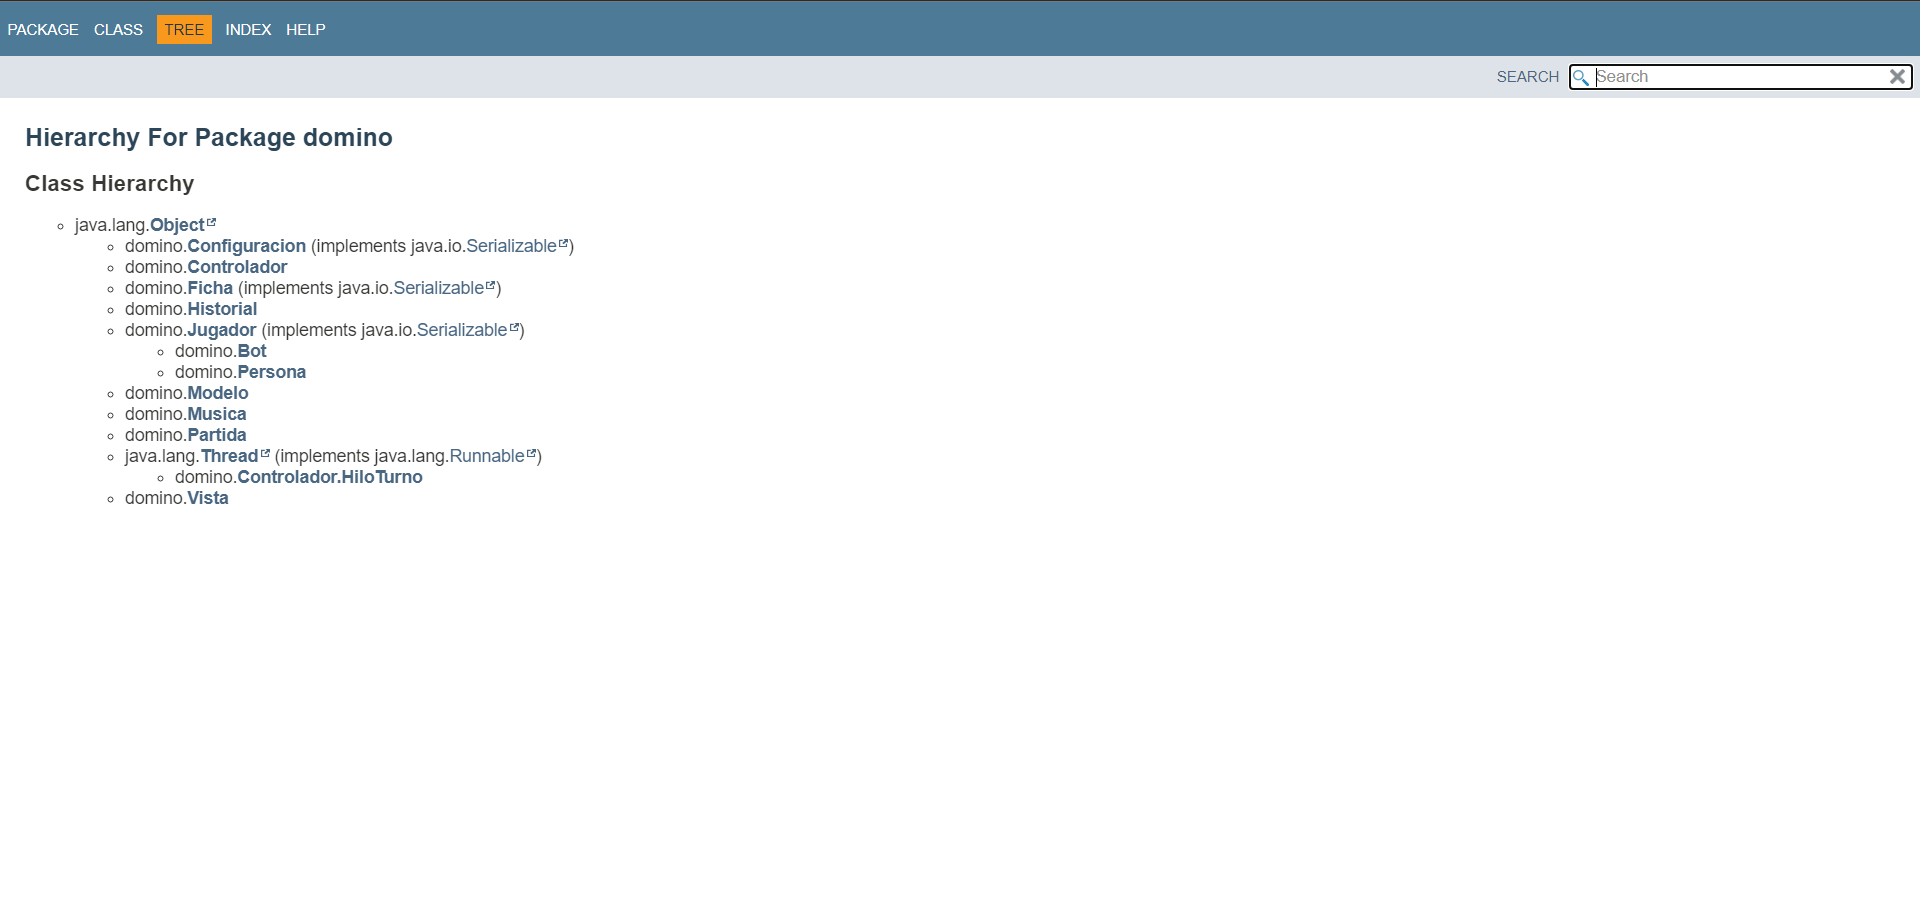
\includegraphics[width=\textwidth]{doc2.png}
    \caption{Árbol de jerarquia de clases}
  \end{figure}

  \begin{figure}[h!]
    \centering
    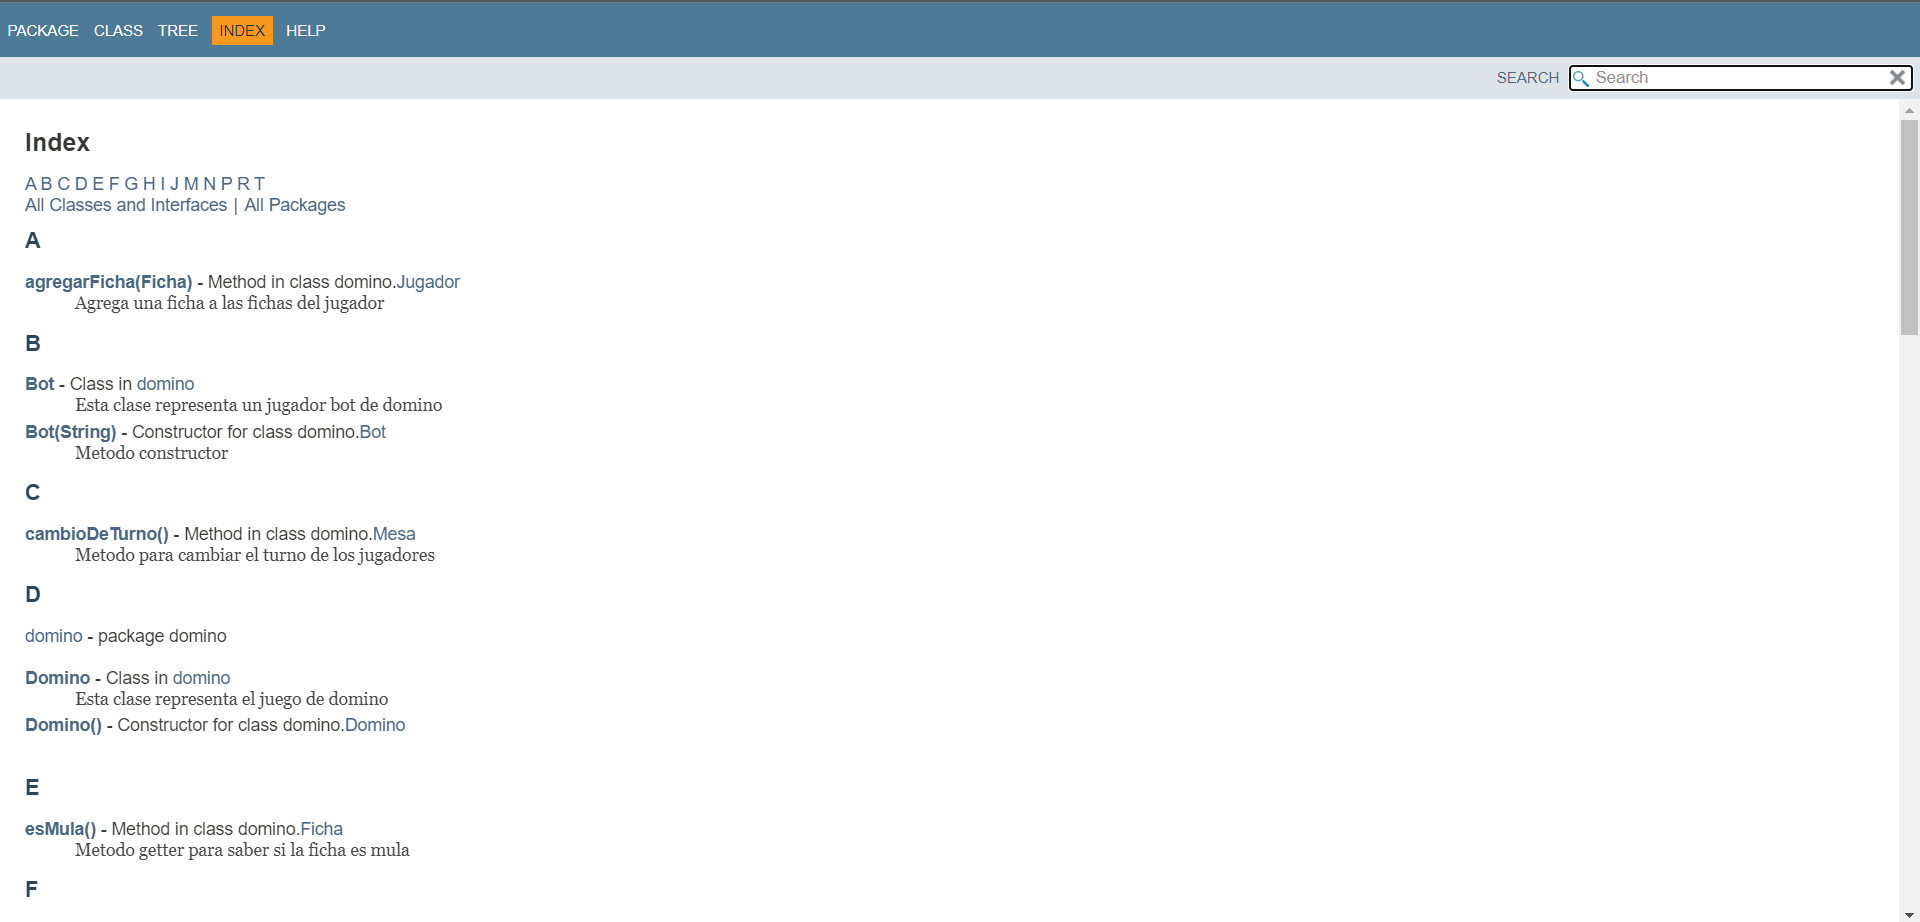
\includegraphics[width=\textwidth]{doc3.png}
    \caption{Índice alfabetico}
  \end{figure}

  \begin{figure}[h!]
    \centering
    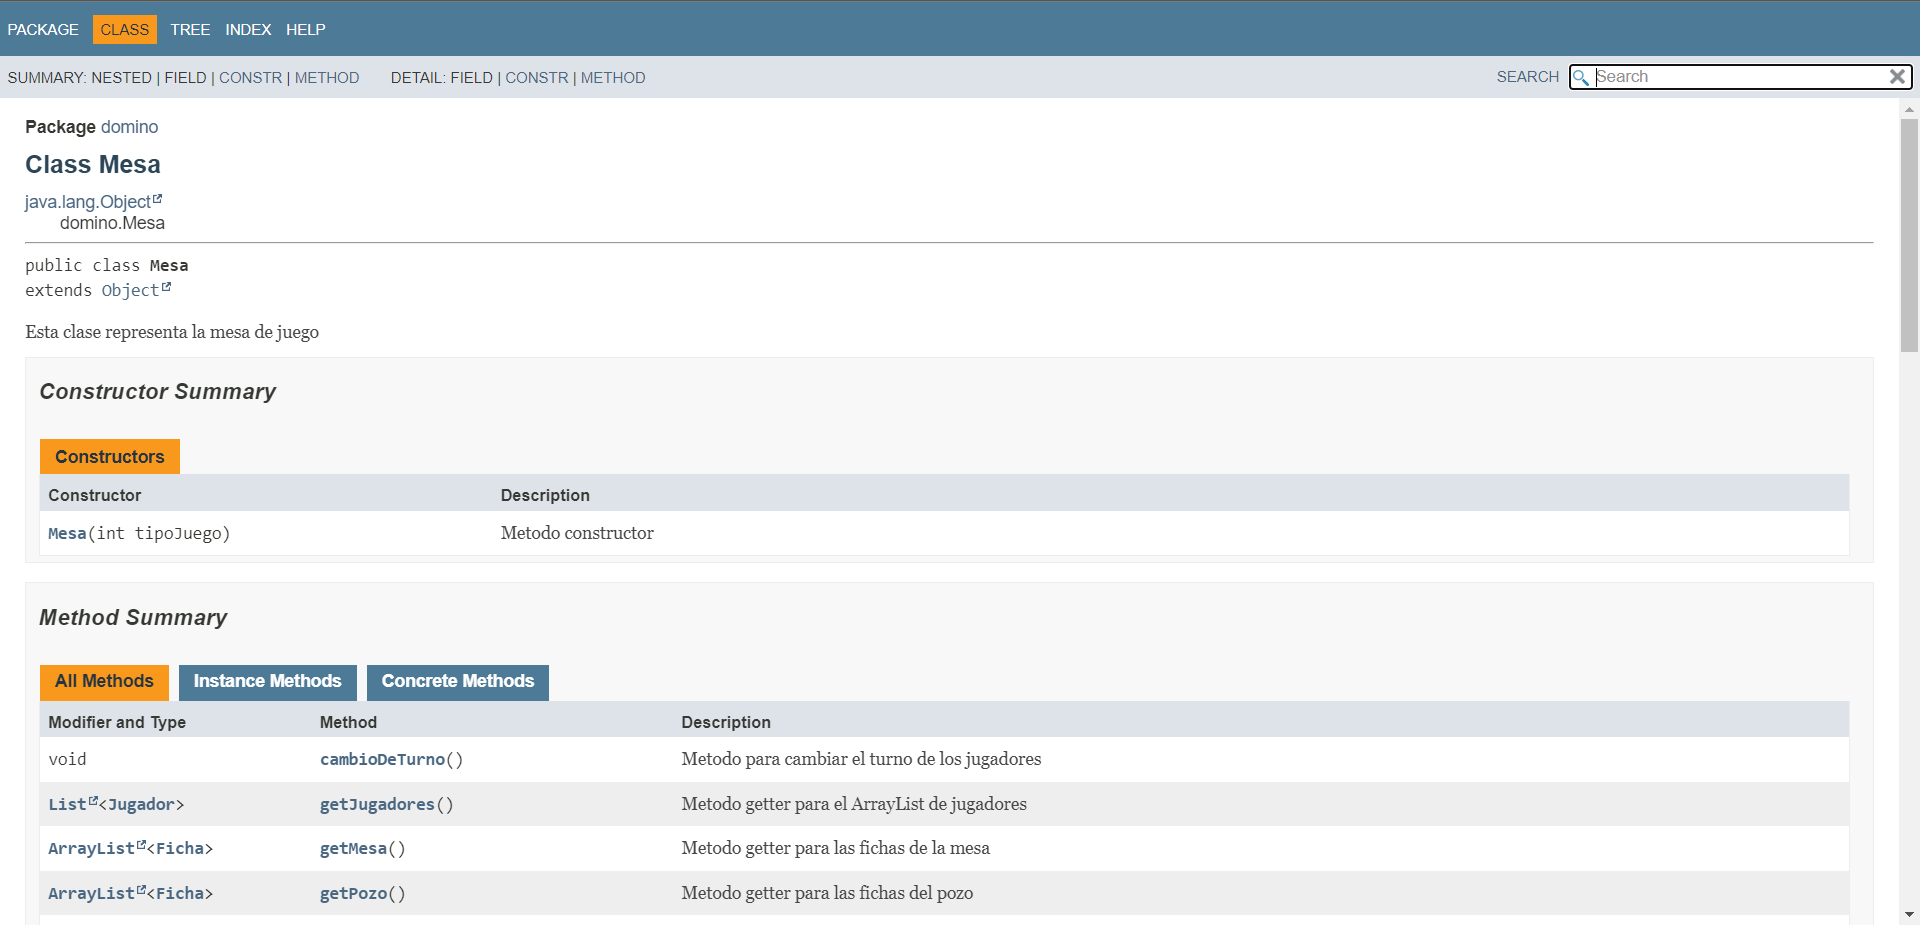
\includegraphics[width=\textwidth]{doc4.png}
    \caption{Página de la clase \textit{Mesa}} 
  \end{figure}
\end{document}